\chapter*{Vedlegg}
\addcontentsline{toc}{chapter}{Appendiks}

\section*{Vedlegg A: Fullstendig fremdriftsplan for masterprosjektet}

Figur~\ref{fig:gantt-full} viser den fullstendige fremdriftsplanen for masterprosjektet, fra innledende utvikling av StellAI-applikasjonen til avsluttende skrivearbeid og innlevering. Diagrammet gir en samlet oversikt over hvordan utviklingsoppgavene – teknologivalg, registreringsflyt, Azure-integrasjon og håndtering av bilder og metadata – henger sammen med brukerevalueringen og skrivefasen i et iterativt løp.

\begin{landscape}
\begin{figure}[p]
    \centering
    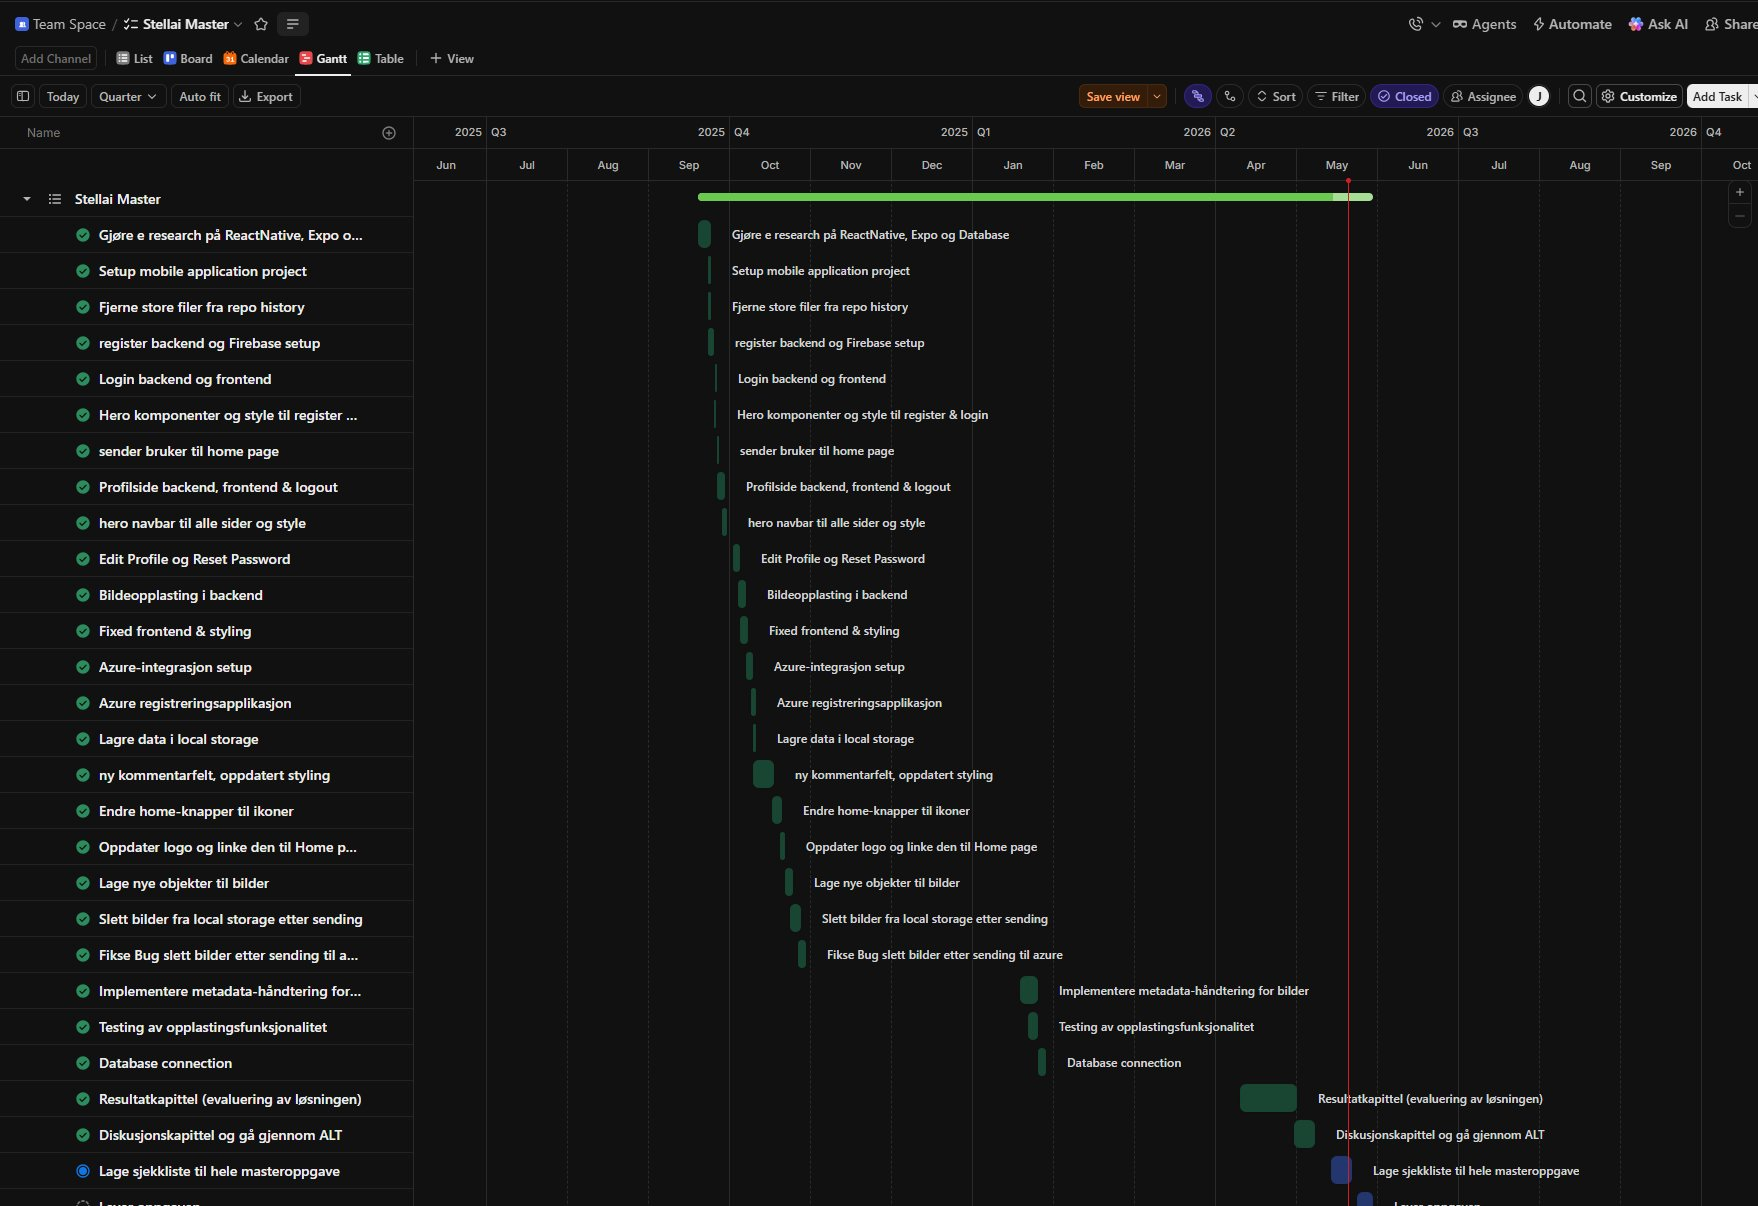
\includegraphics[width=\linewidth]{Figures/Gantt_full_prosjektlop.png}
    \caption{Fullstendig fremdriftsplan for masterprosjektet, fra innledende utvikling av StellAI-applikasjonen til avsluttende skrivearbeid og innlevering. Diagrammet viser hvordan utviklingsoppgavene, brukerevalueringen og skrivefasen henger sammen i et iterativt løp.}
    \label{fig:gantt-full}
\end{figure}
\end{landscape}